
\section{Невронски мрежи}

Имплементација на алгоритмот за повратна пропагација за учење на параметрите на
невронската мрежа. Овој алгоритам ќе го искористиме за препознавање на ракописно
напишани цифри. Ова е корисно во автоматско читање на поштенски кодови, чекови,
сметки и слично.

\subsection{Визуелизација на податоците}

\begin{figure}[htb]
\centering
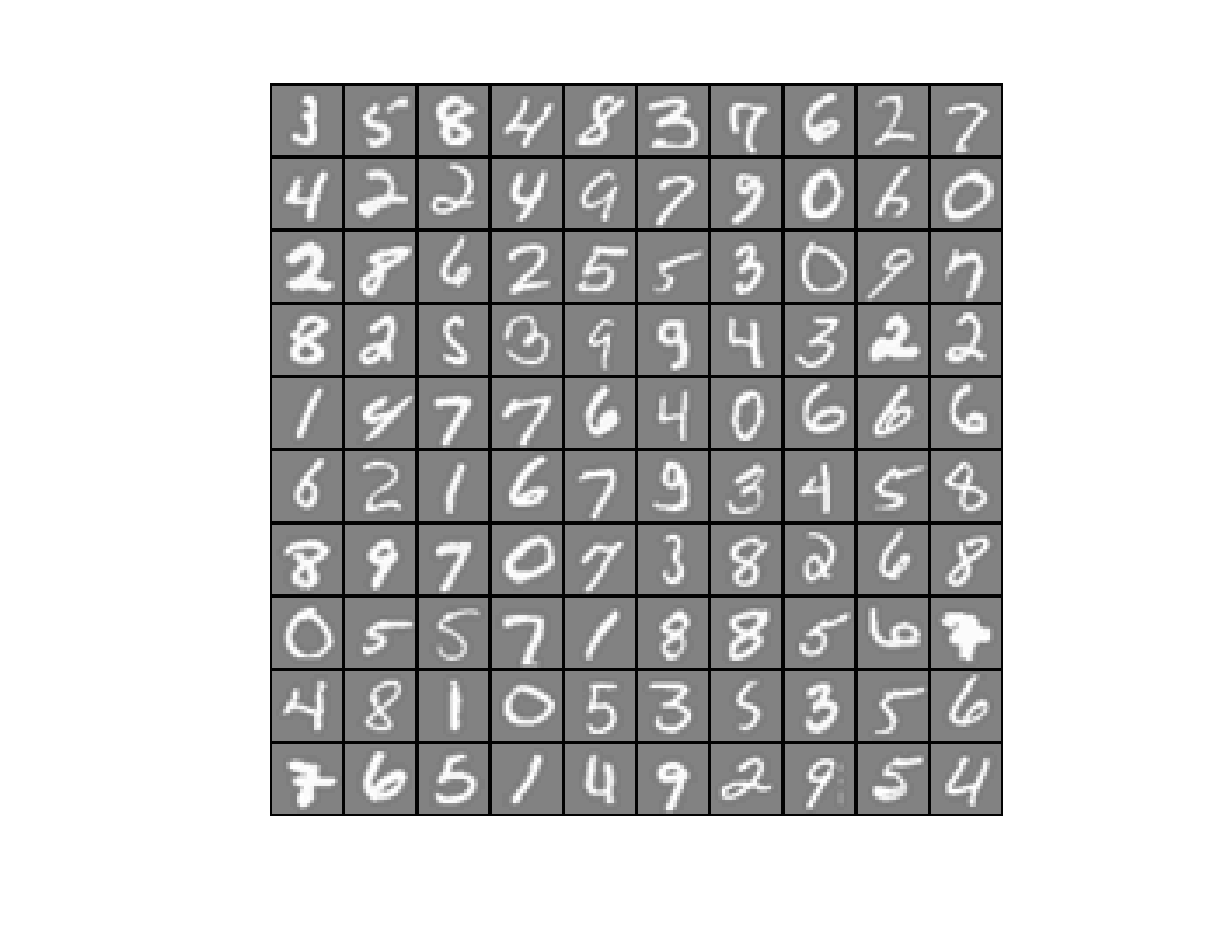
\includegraphics[width=.9\textwidth]{src/neuralNetwork2/nn}
\caption{Примероци од податочното множество}
\label{fig:neuralNetworkData}
\end{figure}

Податочното множество (дел е прикажан на слика \ref{fig:neuralNetworkData}) за овој алгоритам е
составено од 5000 тренинг примероци, од кој секој примерок е црно-бела слика од 20x20 пиксели. Секој пиксел се
репрезентира со децимален број кој го означува интензитетот. Овие 400 пиксели се
сместени во еднодимензионален вектор. Секој од овие тренинг примероци
претставува ред од матрицата X. Со ова се добива матрица од 5000 по 400 во која
секој ред е примерок за слика од ракописно напишана цифра.

\[
	X = \begin{bmatrix}
		    (x^{(1)})^T \\
			(x^{(2)})^T \\
			\vdots \\
			(x^{(m)})^T
			
		\end{bmatrix}
\]

Вториот дел од податочното множество е 5000-димензионален вектор $y$ кој 
ги содржи целните ознаки за податочното множество. За да се постигне
компатибилност со индексирањето во Octave/Matlab, каде што не постои 0 индекс,
цифрата 0 е пресликана во вредноста 10. Така, цифрата „0“ е означена како „10“,
додека цифрите од „1“ до „9“ се означени како „1“ до „9“ во нивниот природен
редослед.

\subsection{Репрезентација на моделот}

\begin{figure}[htb]
\centering
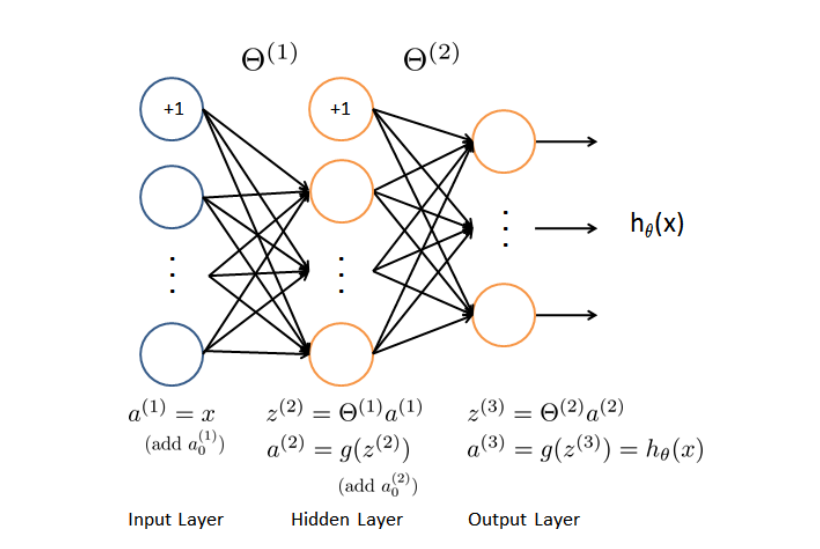
\includegraphics[width=.9\textwidth]{src/neuralNetwork2/neuralNetwork}
\caption{Моделот на невронска мрежа}
\label{fig:neuralNetwork}
\end{figure}

На слика \ref{fig:neuralNetwork} е прикажан моделот на невронската мрежа. Се
состои од 3 слоеви: влезен слој, скриен слој и излезен слој. На влезот на оваа
невронска мрежа се дигиталните слики. Затоа што секоја слика е со големина 20 x
20, влезниот слој е составен од 400 влезни единици.

\subsection{Feedforward propagation and prediction}

fp ја пресметува $h_\theta(x^{(i)})$ за секој примерок $i$ и ја враќа
предвидената вредност. Слично како кај стратегијата за класификација
еден-против-сите, предвидувањето на невронската мрежа ќе биде ознаката со
најголема вредност $(h_\theta(x))_k$.

\lstinputlisting[firstline=6,lastline=17,caption=Имплементација
на функцијата predict]{src/neuralNetwork1/predict.m}


\subsection{feedforward and cost function}

Функцијата на чинење на невронска мрежа (без регуларизација) е

\[
	J(\theta) = \frac{1}{m}\sum_{i = 1}^{m}\sum_{k =
	1}^{K}[-y^{(i)}_k\log((h_\theta(x^{(i)}))_k) -
	(1 - y^{(i)}_k)\log(1 - (h_\theta(x^{(i)}))_k)],
\]

каде што $h_\theta(x^{(i)})$ се пресметува како на слика \ref{fig:neuralNetwork}
 и $K = 10$ е бројот на можни ознаки. Со $(h_\theta(x^{(i)}))_k = a^{(3)}_k$ се
 означува активацијата (излезната вредност) на $k-th$ излезна единица.
 Оригиналните вредности за излезната ознака $y$ се 1, 2, \ldots, 10, за
 тренирање на невронска мрежа, треба сите ознаки да се претворат во соодветни
 вектори кои ги содржат единствено вредностите 0 и 1:
 
 \[	
	y = \begin{bmatrix}
		    1 \\
			0 \\
			0 \\
			\vdots \\
			0
			
		\end{bmatrix},
		\begin{bmatrix}
		    0 \\
			1 \\
			0 \\
			\vdots \\
			0
			
		\end{bmatrix},
		\ldots
		or
		\begin{bmatrix}
		    0 \\
			0 \\
			0 \\
			\vdots \\
			1
			
		\end{bmatrix}
 \]

На пример, ако $x(i)$ е слика од цифрата 5, тогаш соодветното $y(i)$ (кое треба
да се искористи во функцијата на чинење) треба да биде 10-димензионален вектор
со $y_5 = 1$, а останатите елементи 0.

\lstinputlisting[firstline=17,lastline=60,caption=Имплементација
на функцијата на
чинење,basicstyle=\ttfamily\scriptsize]{src/neuralNetwork2/nnCostFunction.m}

\subsection{Backpropagation}

\subsubsection{Сигмоид градиент}

Градиентот за сигмоид функцијата се пресметува како

\[
	g'(z) = \frac{d}{dz}g(z) = g(z)(1 - g(z))
\]

каде што

\[
	sigmoid(z) = g(z) = \frac{1}{1 + e^{-z}}.
\]

\subsubsection{Случајна иницијализација}

Кога се тренираат невронски мрежи, важно е да параметрите да се иницијализираат
случајно за да се наруши симетријата. Една ефективна стратегија за случајна
иницијализација е случајно да се изберат вредности за $\theta(l)$ рамномерно во
опсегот $[-\epsilon_{init}, \epsilon_{init}]$. Овој опсег не осигурува дека
вредностите на параметрите ќе бидат мали, а со тоа и учењето ќе биде поефикасно.

\lstinputlisting[firstline=14,lastline=16,caption=Имплементација
на случајна иницијализација]{src/neuralNetwork2/randInitializeWeights.m}

\subsubsection{Backpropagation}

\begin{figure}[htb]
\centering
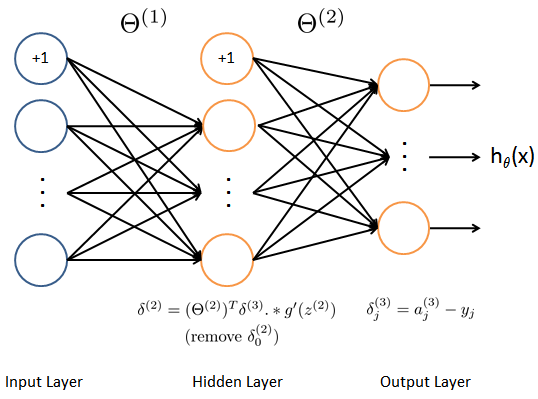
\includegraphics[width=.9\textwidth]{src/neuralNetwork2/nnb}
\caption{Освежување на вредностите во Backpropagation}
\label{fig:backpropagation}
\end{figure}

